\documentclass{article}
\usepackage[utf8]{inputenc}
\usepackage[margin = 0.8in]{geometry}
\usepackage{graphicx}
\usepackage{amsmath, amssymb}
\usepackage{subcaption}
\usepackage{multirow}
\usepackage{mathtools}
\usepackage{float}


\title{RBE502 - Homework Set 5}
\author{Keith Chester}
\date{Due date: September 29 2021}

\begin{document}
\maketitle

\section*{Introduction}

In this homework, we consider a system of an inverted pendulum on a cart, pictured below.

\begin{figure}[H]
    \centering
    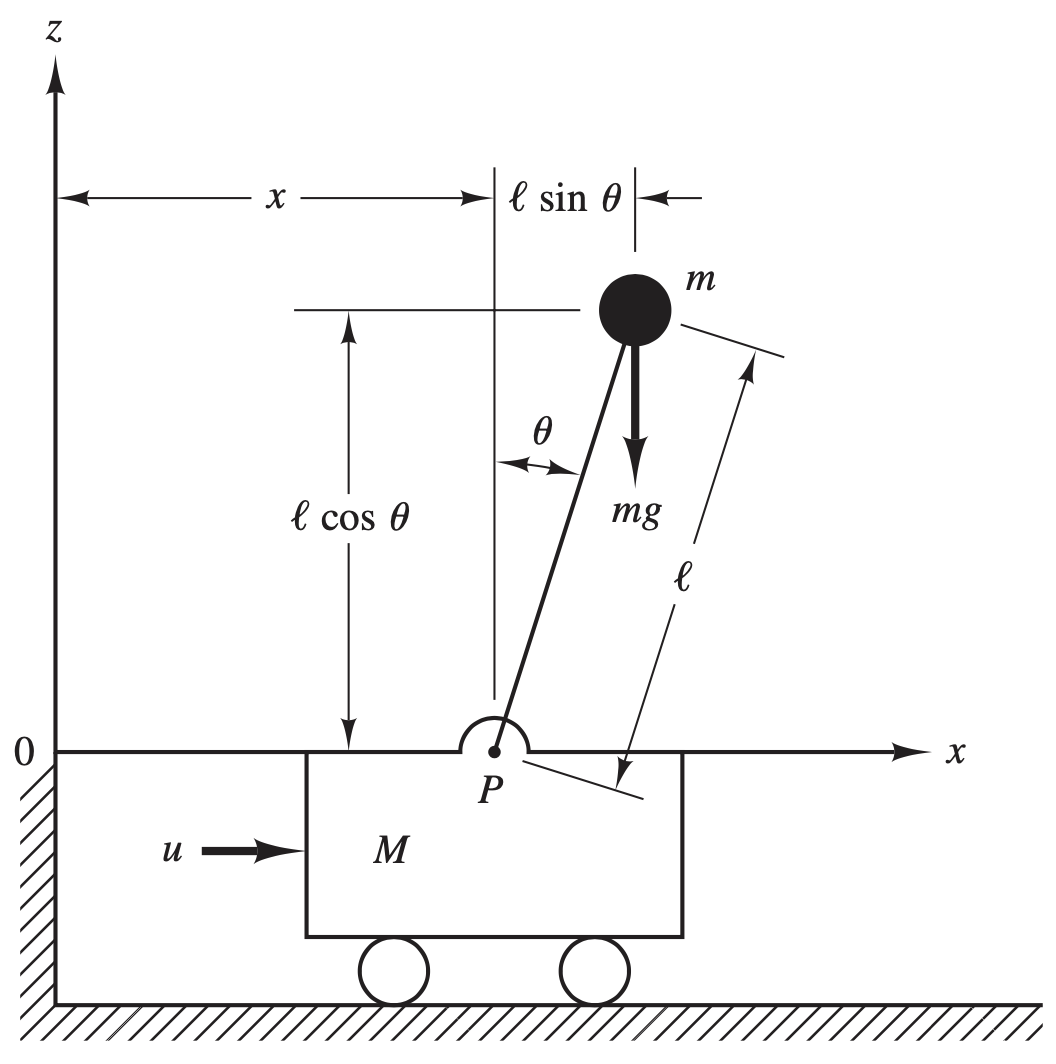
\includegraphics[width = 0.4\textwidth]{figures/cart-pole.png}
    \caption{An inverted pendulum situated atop a cart}
    \label{fig:cart-pole}
\end{figure}

If we assume that $|\theta| << 1$, the linearization of the system about $\theta=0$ gives us the following equations:

\begin{equation}
    M\ddot{x} = u-mg\theta
\end{equation}

\begin{equation}
    Ml\ddot{\theta}=(M+m)g\theta-u
\end{equation}

Letting $z = \begin{bmatrix} x & \theta & \dot{x} & \dot{\theta} \end{bmatrix}^T$ denote the state vector of our system, we wish to utilize Ackermann's formula to create a full-state controller for this system.


\section*{Part A}

First, we wish to take the given state vector and equation of the system, and generate the state-space representation of the system. With the equations already provided, we can create our $\dot{\boldsymbol{z}}$ by rearranging the equations and isolating elements that interact with our input $u$.

\begin{equation}
    \dot{\boldsymbol{z}} = \begin{bmatrix}
        \dot{x} \\
        \dot{\theta} \\
        \ddot{x} \\
        \ddot{\theta}
    \end{bmatrix}
    =
    \begin{bmatrix}
        \dot{x} \\
        \dot{\theta} \\[4pt]
        \frac{-mg\theta}{M}+\frac{u}{M} \\[4pt]
        \frac{(M+m)g\theta}{Ml}-\frac{u}{Ml}
    \end{bmatrix}
\end{equation}

From this $\dot{\boldsymbol{z}}$ we can then find the $\boldsymbol{A}$ and $\boldsymbol{B}$ matricies for the equation $\dot{\boldsymbol{z}}=\boldsymbol{A}\boldsymbol{z}+\boldsymbol{B}u$. $\boldsymbol{A}$ is the Jacobian of $\dot{\boldsymbol{z}}$ by $\boldsymbol{z}$, while $\boldsymbol{B}$ is the Jacobian of $\dot{\boldsymbol{z}}$ by $u$. Thus:

\begin{equation}
    \boldsymbol{A} = \begin{bmatrix}
        \frac{\partial \dot{x}}{\partial x} &
        \frac{\partial \dot{x}}{\partial \theta} &
        \frac{\partial \dot{x}}{\partial \dot{x}} &
        \frac{\partial \dot{x}}{\partial \dot{\theta}}
        \\[4pt]
        \frac{\partial \dot{\theta}}{\partial x} &
        \frac{\partial \dot{\theta}}{\partial \theta} &
        \frac{\partial \dot{\theta}}{\partial \dot{x}} &
        \frac{\partial \dot{\theta}}{\partial \dot{\theta}}
        \\[4pt]
        \frac{\partial \ddot{x}}{\partial x} &
        \frac{\partial \ddot{x}}{\partial \theta} &
        \frac{\partial \ddot{x}}{\partial \dot{x}} &
        \frac{\partial \ddot{x}}{\partial \dot{\theta}} 
        \\[4pt]
        \frac{\partial \ddot{\theta}}{\partial x} &
        \frac{\partial \ddot{\theta}}{\partial \theta} &
        \frac{\partial \ddot{\theta}}{\partial \dot{x}} &
        \frac{\partial \ddot{\theta}}{\partial \dot{\theta}}
        \\[4pt]
    \end{bmatrix}
    =
    \begin{bmatrix}
        0 & 0 & 1 & 0\\
        0 & 0 & 0 & 1\\[4pt]
        0 & -\frac{g\,m}{M} & 0 & 0\\[4pt]
        0 & \frac{g\,{\left(M+m\right)}}{M\,l} & 0 & 0
    \end{bmatrix}
\end{equation}
\begin{equation}
    \boldsymbol{B} = \begin{bmatrix}
        \frac{\partial \dot{x}}{\partial x}
        \\[4pt]
        \frac{\partial \dot{\theta}}{\partial x}
        \\[4pt]
        \frac{\partial \ddot{x}}{\partial x}
        \\[4pt]
        \frac{\partial \ddot{\theta}}{\partial x}
        \\[4pt]
    \end{bmatrix}
    =
    \begin{bmatrix}
        0\\
        0\\[4pt]
        \frac{1}{M}\\[4pt]
        -\frac{1}{M\,l}
    \end{bmatrix}
\end{equation}

From these we can construct our system equation $\dot{\boldsymbol{z}}=\boldsymbol{A}\boldsymbol{z}+\boldsymbol{B}u$ as:

\begin{equation}
    \begin{bmatrix}
        \dot{x} \\ \dot{\theta} \\ \ddot{x} \\ \ddot{\theta}
    \end{bmatrix}
    =
    \begin{bmatrix}
        0 & 0 & 1 & 0\\
        0 & 0 & 0 & 1\\[4pt]
        0 & -\frac{g\,m}{M} & 0 & 0\\[4pt]
        0 & \frac{g\,{\left(M+m\right)}}{M\,l} & 0 & 0
    \end{bmatrix}
    \begin{bmatrix}
        x \\ \theta \\ \dot{x} \\ \dot{\theta}
    \end{bmatrix}
    +
    \begin{bmatrix}
        0\\
        0\\[4pt]
        \frac{1}{M}\\[4pt]
        -\frac{1}{M\,l}
    \end{bmatrix}
    u
\end{equation}

We can now compute the eigenvalues of $\boldsymbol{A}$ for our equilibrium point of $(\boldsymbol{z}=0, u=0)$. The calculated eigenvalues are shown below:

\begin{equation}
    \sigma(\boldsymbol{A}) =
    \begin{bmatrix}
        0\\
        0\\[4pt]
        -\sqrt{\frac{g\,{\left(M+m\right)}}{M\,l}}\\[4pt]
        \sqrt{\frac{g\,{\left(M+m\right)}}{M\,l}}
    \end{bmatrix}
\end{equation}

Here we see that we have a positive and negative eigenvalue for our $\boldsymbol{A}$ matrix. As a result, we know that the system is an unstable saddle point. This makes sense if we pause to imagine the inverted pendulum we're working with; while it is possible to balance the pendulum vertically, any slight pertubation will cause the pendulum to fall away from that equilibrium point.

\section*{Part B}

Now we wish to use Ackermann's formula to find a control function $u=-\boldsymbol{K}\boldsymbol{z}$, where $\boldsymbol{K}=\begin{bmatrix}k_1 & k_2 & k_3 & k_4\end{bmatrix}$ such that $\sigma(\hat{\boldsymbol{A}})$. Per Ackermann's formula, $\hat{\boldsymbol{A}} = \boldsymbol{A}-\boldsymbol{B}\boldsymbol{K}$, for a state equation of $\dot{\boldsymbol{z}} = (\boldsymbol{A}-\boldsymbol{B}\boldsymbol{K})\boldsymbol{z} = \hat{\boldsymbol{A}}\boldsymbol{z}$. We are looking to use $\sigma(\hat{\boldsymbol{A}}) = \begin{bmatrix}
    -5 &
    -4 &
    -3+2i &
    -3-2i
\end{bmatrix}$.

First, we need to check to see if the system is controllable. To do this, we can solve for a matrix $\boldsymbol{C}$ such that $
    \boldsymbol{C} = \begin{bmatrix}
        \boldsymbol{A}^0\boldsymbol{B} & \boldsymbol{A}^1\boldsymbol{B} & \ldots & \boldsymbol{A}^{n-1}\boldsymbol{B}
    \end{bmatrix}$ where $n=4$ for our matrix. If the $rank(\boldsymbol{C})=n=4$, we know our system is controllable. Thus:

\begin{equation}
    rank(\boldsymbol{C}) = rank(\begin{bmatrix}
        \boldsymbol{A}^0\boldsymbol{B} & \boldsymbol{A}^1\boldsymbol{B} & \boldsymbol{A}^2\boldsymbol{B} & \boldsymbol{A}^3\boldsymbol{B}
    \end{bmatrix}) = 4
\end{equation}

Now that we know our system is controllable, we can continue trying to solve for our desired eigenvalues for the system. Given our eigenvalues, we can set our characteristic equation to:

\begin{equation}
    (\lambda+5)(\lambda+4)(\lambda+3+2i)(\lambda+3-2i)=\lambda^4+15\lambda^3+87\lambda^2+237\lambda+260
\end{equation}

With this characteristic equation and $\boldsymbol{C}$, we can now move to solve for $\boldsymbol{K}$. Note that $\boldsymbol{K}_{selector} =\begin{bmatrix}0 & 0 & 0 & 1\end{bmatrix}$, where the row length $n$ is equal to the number of eigenvalues we started with, with the final column $n$ being set to $1$.  

\begin{equation}
    \boldsymbol{K} = \begin{bmatrix}k_1 & k_2 & k_3 & k_4\end{bmatrix} = \boldsymbol{K}_{selector} \boldsymbol{C}^{-1} \Delta_{new}(\boldsymbol{A})
\end{equation}

\begin{equation}
    \Delta_{new} = \lambda^4+15\lambda^3+87\lambda^2+237\lambda+260\boldsymbol{I}_4
\end{equation}

\begin{equation}
    \Delta_{new}(\boldsymbol{A}) = \boldsymbol{A}^4+15\boldsymbol{A}^3+87\boldsymbol{A}^2+237\boldsymbol{A}+260\boldsymbol{I}_4
\end{equation}

\begin{equation}
    \boldsymbol{K} = \begin{bmatrix}0 & 0 & 0 & 1\end{bmatrix} \boldsymbol{C}^{-1} \Delta_{new}(A) = \begin{bmatrix}
        -\frac{260\,M\,l}{g} & -\frac{M\,g^2 +260\,M\,l^2 +g^2 \,m+87\,M\,g\,l}{g} & -\frac{237\,M\,l}{g} & -\frac{3\,M\,l\,{\left(5\,g+79\,l\right)}}{g}
    \end{bmatrix}
\end{equation}

\begin{equation}
    \hat{\boldsymbol{A}} = \boldsymbol{A} - \boldsymbol{B}\boldsymbol{K} = \begin{bmatrix}
        0 & 0 & 1 & 0 \\
        0 & 0 & 0 & 1 \\[4pt]
        \frac{260l}{g} & g+87l+\frac{260l^2}{g} & \frac{237l}{g} & 15l + \frac{237l^2}{g} \\[4pt]
        \frac{-260}{g} & -87+\frac{260l}{g} & \frac{-237}{g} & 15 - \frac{237l}{g} \\[4pt]
    \end{bmatrix}
\end{equation}

Finally, we can solve for our system utilizing our new $\boldsymbol{K}$ and resulting $\hat{\boldsymbol{A}}$ to solve our equation for $\dot{\boldsymbol{z}} = \hat{\boldsymbol{A}}\boldsymbol{z}$.

\begin{equation}
    \begin{bmatrix}
        \dot{x} \\ \dot{\theta} \\ \ddot{x} \\ \ddot{\theta}
    \end{bmatrix}
    =
    \begin{bmatrix}
        0 & 0 & 1 & 0 \\
        0 & 0 & 0 & 1 \\[4pt]
        \frac{260l}{g} & g+87l+\frac{260l^2}{g} & \frac{237l}{g} & 15l + \frac{237l^2}{g} \\[4pt]
        \frac{-260}{g} & -87+\frac{260l}{g} & \frac{-237}{g} & 15 - \frac{237l}{g} \\[4pt]
    \end{bmatrix}
    \begin{bmatrix}
        x \\ \theta \\ \dot{x} \\ \dot{\theta}
    \end{bmatrix}
\end{equation}

\section*{Part C}

In this section, we wish to investigate the affect that various chosen poles have on the control system's response. We will choose $\sigma(\hat{\boldsymbol{A}})$ to demonstrate and plot the system state over time.

For this we shall choose a range of values expanding out in a Fibonacci growth, specifically $\begin{bmatrix} -1 & -3 & -5 & -8  \end{bmatrix}$, to see varied responses. We shall keep all poles equivalent, \textit{ie} for a value of $n$ all poles shall be set to $n$, for a resulting characteristic equation of $(\lambda-n)^4$. Continuing this example with one of our chosen values, $-1$, we see that $(\lambda+1)^4=\lambda^4+4\lambda^3+6\lambda^2+4\lambda+1$.

Next we take the coeffeicients for these characteristic equations and calculate $\boldsymbol{K}$ similary to above, specifically 

\begin{equation}
    \boldsymbol{K} = \boldsymbol{K}_{selector} \boldsymbol{C}^{-1} \Delta_{new}(\boldsymbol{A})
\end{equation}

\noindent...and continue on to solve our new $\hat{\boldsymbol{A}} = \boldsymbol{A} - \boldsymbol{B}\boldsymbol{K}$. With this, we can use MATLAB's $ode45$ solver to calculate how the system state responds with the given control system over a set period of time - for our purposes we looked at 10 seconds. We used an initial state of $z_0=\begin{bmatrix}x & \theta & \dot{x} & \dot{\theta} \end{bmatrix}=\begin{bmatrix} 0 & 0.5 & 0 & 0 \end{bmatrix}$. This initial value is chosen to have the inverted pendulum be slightly off tilt. We do not wish for the system to start perfectly balanced, as it will simply stay in equilibrium.

The results of our experiments are plotted below:


 
\begin{figure}[H]
    \centering
    \begin{subfigure}{0.45\textwidth}
        \centering
        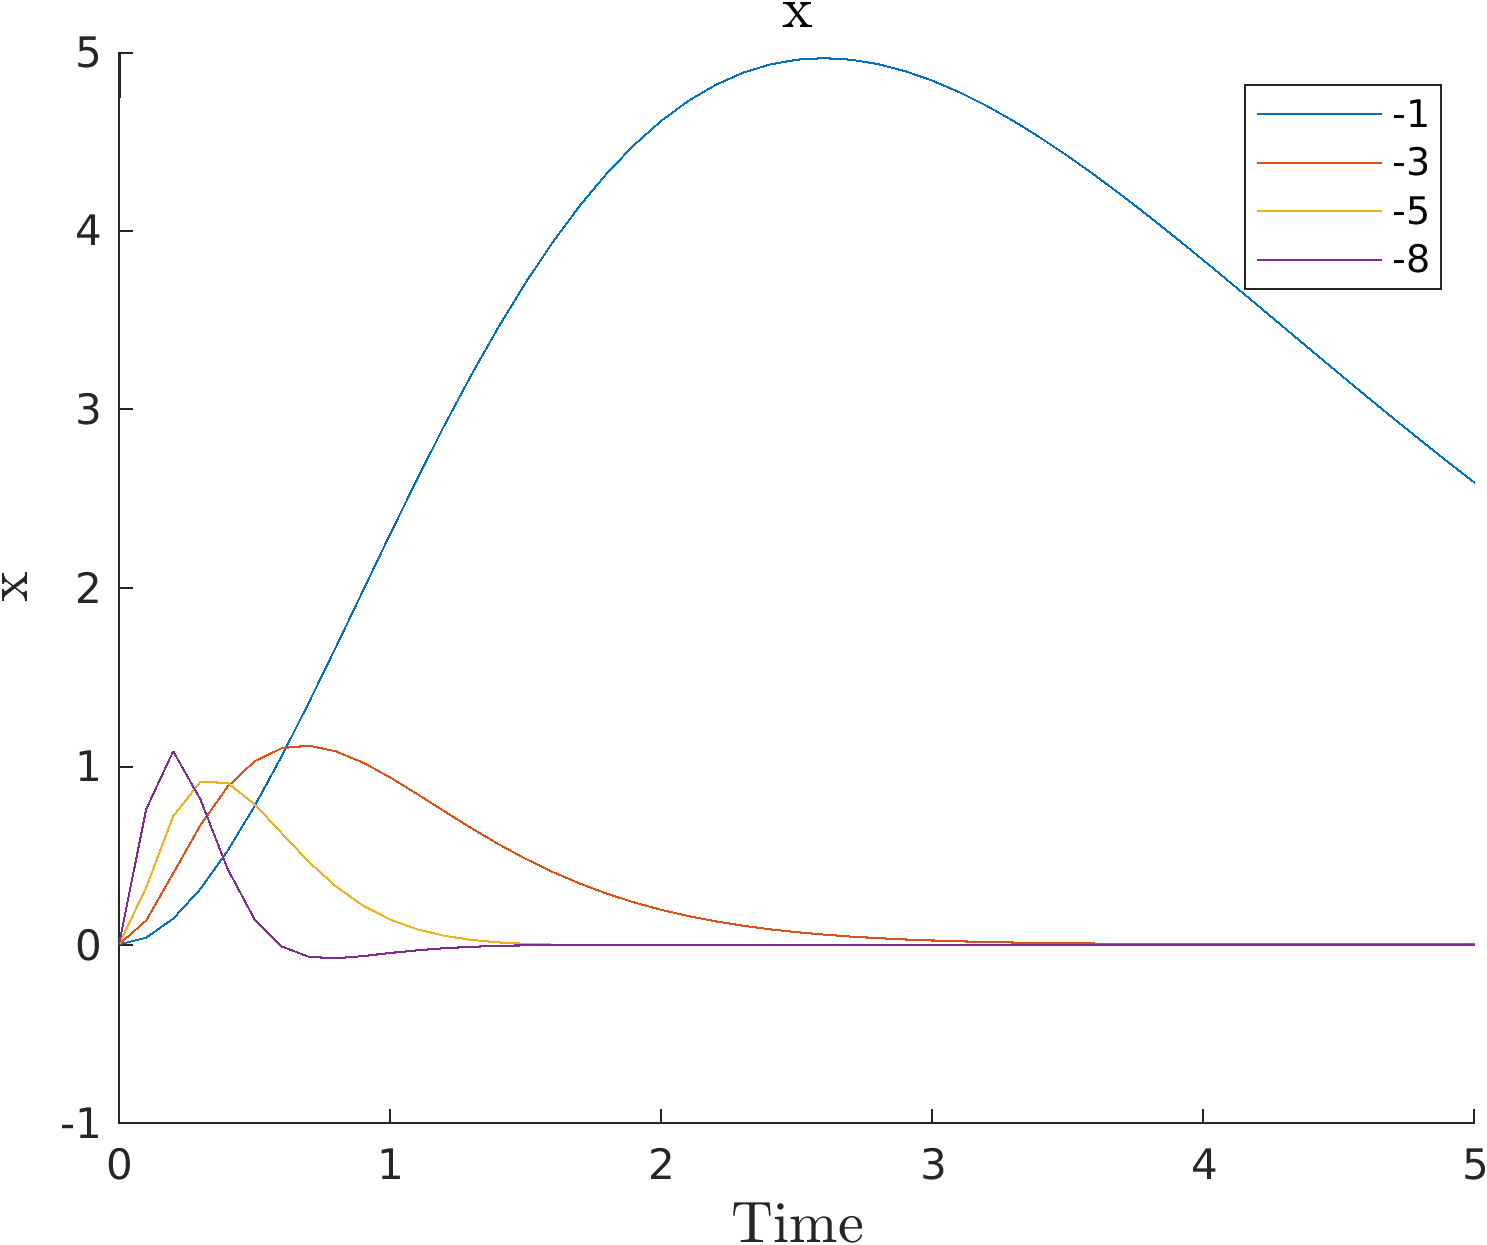
\includegraphics[width = \textwidth]{figures/x_plot.png}
        \caption{x position}
    \end{subfigure}
    \begin{subfigure}{0.45\textwidth}
        \centering
        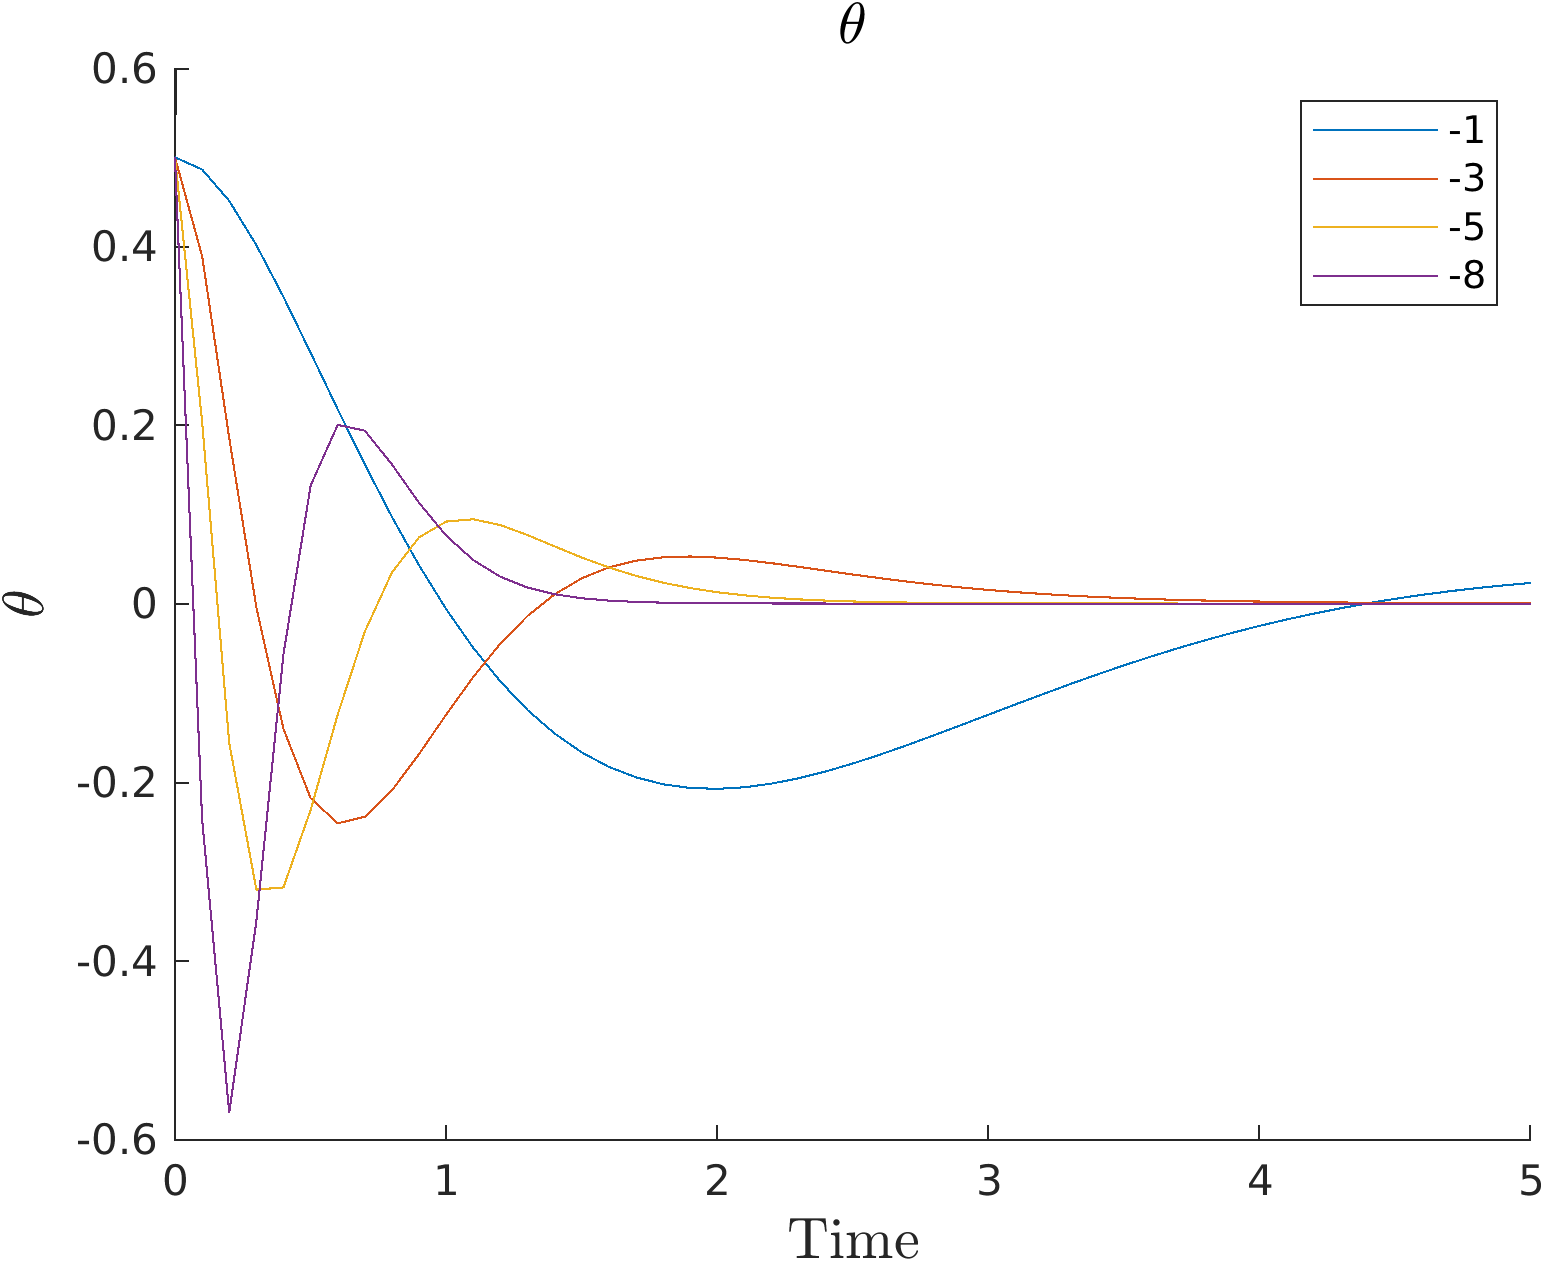
\includegraphics[width = \textwidth]{figures/theta_plot.png}
        \caption{$\theta$ orientation}
    \end{subfigure}
    \begin{subfigure}{0.45\textwidth}
        \centering
        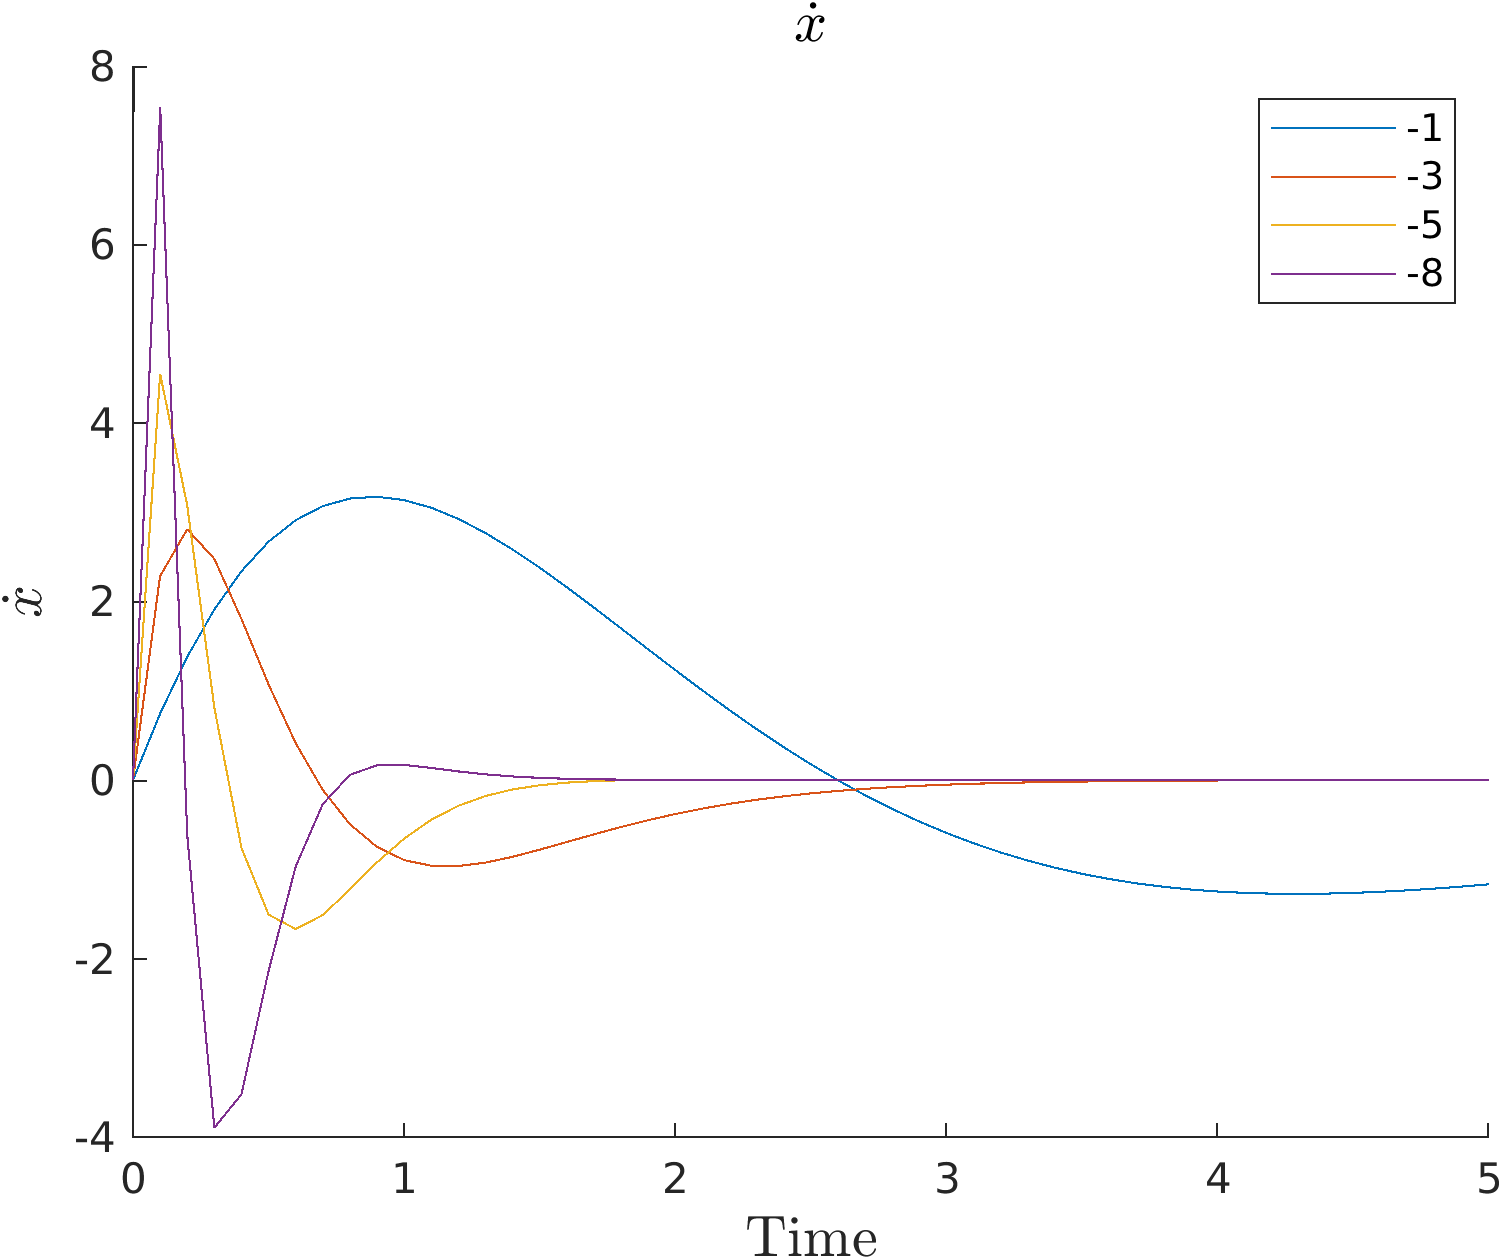
\includegraphics[width = \textwidth]{figures/xdot_plot.png}
        \caption{Change in x position}
    \end{subfigure}
    \begin{subfigure}{0.45\textwidth}
        \centering
        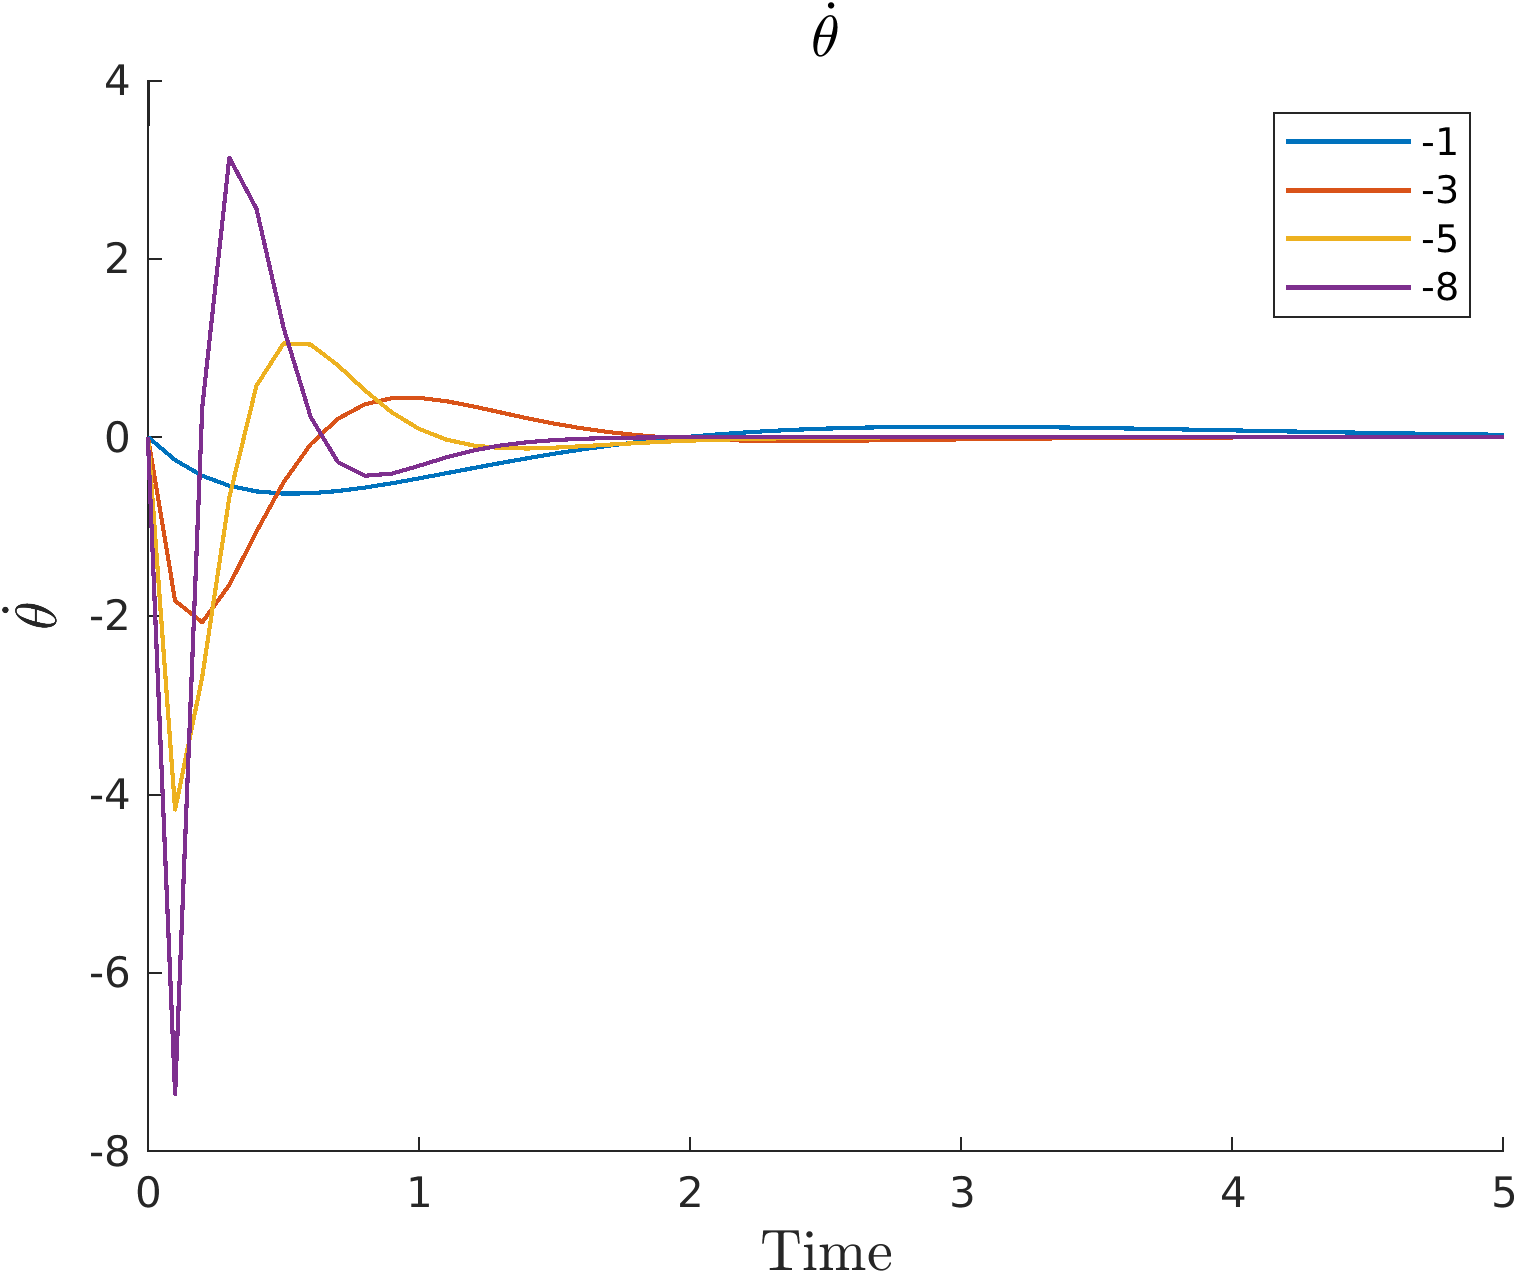
\includegraphics[width = \textwidth]{figures/thetadot_plot.png}
        \caption{Change in $\theta$ orientation}
    \end{subfigure}
    \caption{Varying $\sigma(\hat{\boldsymbol{A}})$ for multiple systems and their responses over 5 seconds}
    \label{fig:part-2_results}
\end{figure}

Our control system is moving the cart to try and maintain the steady state of our system $z=\begin{bmatrix}x & \theta & \dot{x} & \dot{\theta} \end{bmatrix}=\begin{bmatrix} 0 & 0 & 0 & 0 \end{bmatrix}$. We see that with poles of $\sigma(\hat{\boldsymbol{A}})$ set to all $-1$, the system does not actually reach a point of equilibrium within the five alotted seconds. Plotting the time further out showed it took above ten seconds for the system to come to an equilibrium like the other systems. For a system with $\sigma(\hat{\boldsymbol{A}})$ set to $-8$, we see that the system had large swings in its values. It seems that a pole value too low causes the system to respond slowly, whereas a pole value that is too high will cause large swings but a faster overall response to changes in the system. Either could be problematic for a real word system - the lower value could produce a system that reaches equilibrium too slowly, or doesn't react to strong enough pertubations in the system. Alternatively the harsh response of the higher value of the system seems to create violent changes that, if converted to accelerations with a real mass, could produce undesired responses in our system.


\end{document}